\chapter{Lecture 20}
\section{Model-Data Interaction}
We continue our discussion on model-data interaction. Consider the following ODE.
\begin{ceqn} \label{eqn:20:ode}
\frac{du}{dx} &= a(x) u(x) +  b(x) \\
u(0) &= u_0
\end{ceqn}
In the context of solving this ODE, our data are the parameters $a,b,u_0$. In the context of solving the inverse problem for this ODE, our data is the solution $Bu(x)$ where $B$ is an observation operator and $u$ is the solution to the ODE, and our output are the parameters $a,b,u_0$ (or some subset of these three, assuming that the others are known). The observation operator $B$ expresses the limits of our ability to observe the whole solution $u(x)$ in practice. For example, $Bu(x) = \{u(x_0),...,u(x_n)\}$ where $x_0,...,x_n$ live on a finite-element grid, recalling that FEM is able to find the exact values of the solution at the nodes.
\askbjorn{We seem to jump to interpolation of functions; should this be a subsection or its own section? Interpolation of functions seems to relate to the comment regarding observation operators}

\subsection{Interpolation in One Dimension}
In lieu of our previous comment, our goal is to find a continuous field given given data. This task is referred to as \bt{interpolation}. That is, given $\{f_j\}_{j=1}^{J}$ for grid points $\{x_1,..,x_J\}$ to approximate a model function $f(x)$. For simplicity, we assume that $f_j=f(x_j)$ is exactly for each $j$, which in the context of finite-element methods is the case (modulo floating point error). A few methods of interpolation are given below.

\begin{center}
\begin{enumerate}
    \item Polynomial interpolation \label{eqn:20:polyint}
    \item Piecewise polynomial interpolation \label{eqn:20:pcwpoly}
    \item Trigonometric interpolation \label{eqn:20:trigint}
    \item Kriging \label{eqn:20:krig}
    \item Other bases, e.g. wavelets \label{eqn:20:other}
\end{enumerate}
\end{center}
\tcr{figure out how to center this list}

\subsubsection{Polynomial interpolation}
Polynomial interpolation is based on the following theorem.
\begin{theorem}{(Polynomial interpolation)} \label{thm:20:polyint}
Let $\{(x_j,y_j)\}_{j=1}^{J}$ be a set of points with $x_j \neq x_k$ when $j \neq k$. Then there exists a unique polynomial $p$ of degree at most $J-1$ such that $p(x_j) = y_j$. 
\end{theorem}
The main advantage of polynomial interpolation is that the solution is analytic. However, the interpolation is extremely sensitive to perturbations and is thus, in general, not the best approach to interpolation. This sensitivity is referred to as \bt{Runge's phenomenon}. Consider the interval $I = [-1,1]$ and define the \bt{Runge function} $f : I \to \R$ by
\begin{align} \label{eqn:20:rungefnc}
f(x) = \frac{1}{1 + 25x^2}. 
\end{align}
Let $\mathcal{G}_{n} = \{x_0, x_1, ..., x_n\}$ with $x_j = -1 + \frac{2i}{n}$ be a uniform grid of $[-1,1]$ with $n+1$ points. Let $p_n$ be the interpolating polynomial given by Theorem \ref{thm:20:polyint}. Carl Runge showed the following result in 1901.
\begin{align} 
\lim_{n \to \infty} \|f - p_{n}\|_{L^{\infty}(I)} = \infty.
\end{align}
As $n \to \infty$, oscillations near the right endpoint get faster and larger, and this is what leads to this result. This is illustration in Figure \ref{fig:20:rungephen} which shows reasonable results up to degree $10$ and complete deterioritation of the approximation by degree $20$.
\begin{figure}
    \centering
    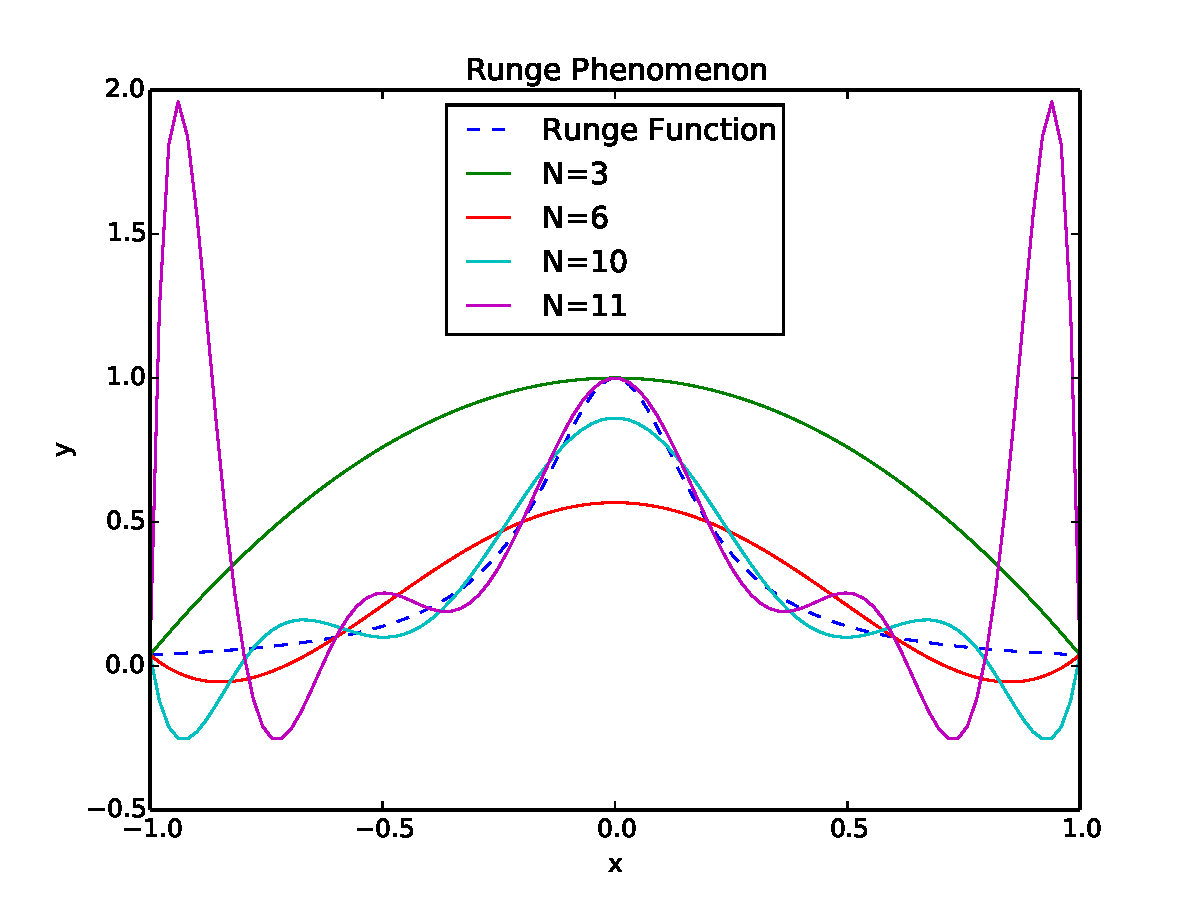
\includegraphics[width=\textwidth]{images/runge11.pdf}
    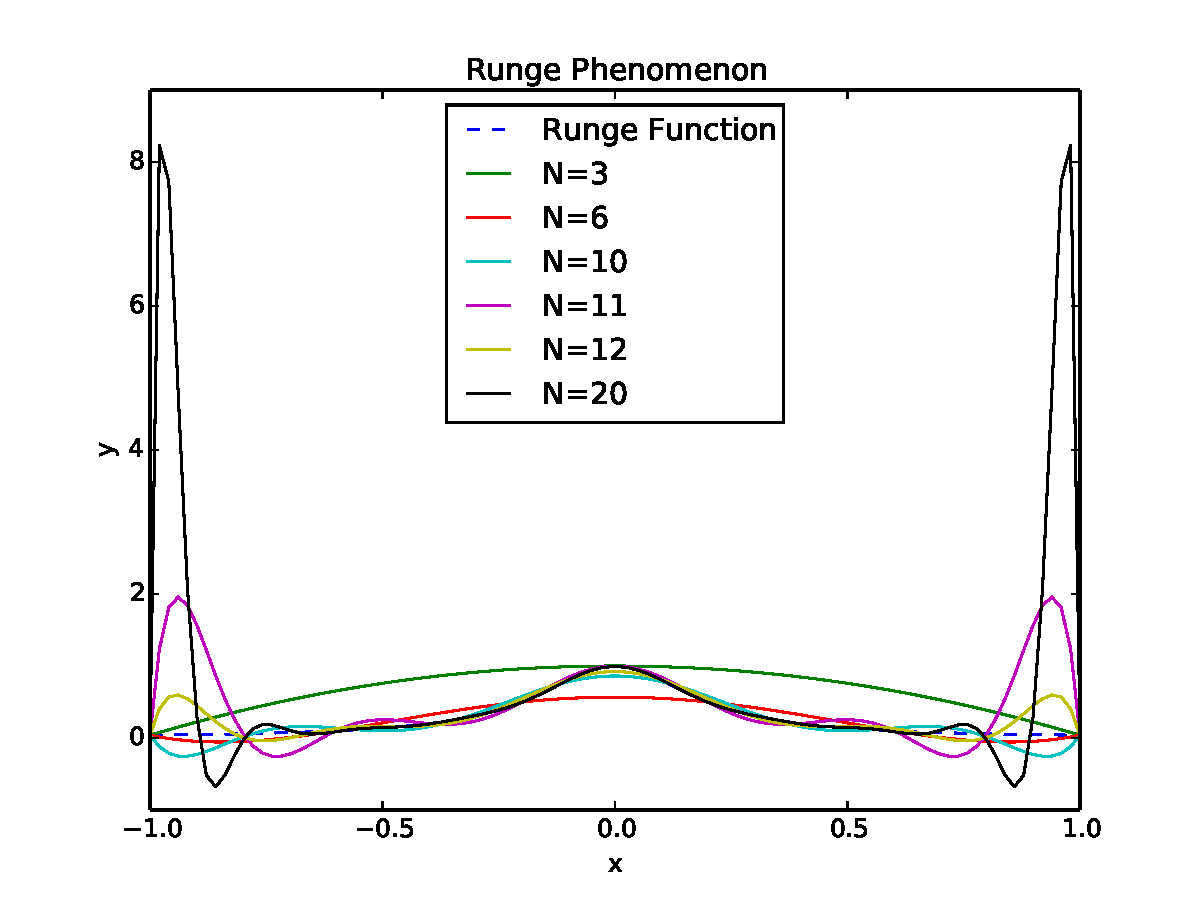
\includegraphics[width=\textwidth]{images/runge20.pdf}
    \caption{Increasing oscillation magnitude near the endpoints.}
    \label{fig:20:rungephen}
\end{figure}
Runge's phenomenon motivates the use of piecewise polynomial interpolation.

\subsubsection{Piecewise Polynomial Interpolation}
Instead of globally approximating our function $f$ by a polynomial, we approximate $f$ piecewise by multiple polynomials. The major advantage of this approach is that in contrast to global polynomial interpolation, piecewise polynomial interpolation is stable with respect to perturbations. The major disadvantages of this approach is that regularity at interfaces is lost and that a larger linear system of equations must be solved to extract coefficients for the polynomials. However, both of these issues can be worked around to some degree. B-splines are a type of piecewise polynomial which allows for control of the smoothness at the interfaces! Furthermore, the linear systems needed to obtain the coefficients can, in certain contexts, be precomputed. \askbjorn{Come up with an example of this; note also that this is a question I posed during class, so the precomputation might not be as strong as I'm interpreting and \bjorn and I had a miscommunication here...it seems to me that the cost of the linear system is essentially negligible since this system could be solved up to say order $30$, which is basically overkill as it is}. 

\subsubsection{Trigonometric Interpolation}
Trigonometric interpolation needs $\{x_j\}$ to be uniformly spaced for efficiency. Constraints to obtain the coefficients are often obtained with either (a) direct formulae or (b) an optimization method such as gradient descent or the Newton-Raphson method.

\subsubsection{Kriging}
We will return to this topic later.

\subsubsection{Other methods}
\askbjorn{Not exactly sure I understand the motivation for the equation I have written down in the iPad.}

\subsection{Interpolation in Higher Dimensions}

